\documentclass{beamer}


% Theme choice
\usetheme{metropolis} 						% You can change this theme to Warsaw, Copenhagen, etc.
\usecolortheme{sidebartab} 					% Adjust color scheme if needed

% Package imports
\usepackage{graphicx} 						% For including images
\usepackage{hyperref}						% For hyperlinks
\usepackage{xcolor} 						% For custom colors
\usepackage{mathptmx}						% Times new roman
\usepackage{booktabs}						% For proffessional tables.
\usepackage{lipsum}
\usepackage[backend=biber, style=authoryear]{biblatex}
\addbibresource{../references.bib} 

% SETTINGS
\setbeamertemplate{headline}{}  			% Remove header
\setbeamertemplate{footline}{}  			% Remove footer
\setbeamertemplate{navigation symbols}{}	% Remove icons from the bottom of the page
%\setmainfont{Times New Roman}

% END SETTINGS

% Title Page
\title{The Physics of Superheroes}
\subtitle{A dummy document to demo Latex}
\author{Samson Rapando}
\date{February 12, 2025}

\begin{document}
	\begin{frame}
		\titlepage
	\end{frame}
	
	\section{Introduction}
	
	\begin{frame}{Introduction to Superheroes}
		\lipsum[1][1-3] \\
		\vspace{1em}
		\lipsum[1][9-11] \parencite{newton1687principia}
	\end{frame}
	
	\section{Spider-Man}
	
	\begin{frame}{Who is Spider-Man?}
		\lipsum[3][4-7]  \parencite{marvel2021spiderman}\\
		\vspace{2em}
		
		\begin{columns}
			\column{0.8\textwidth}
			\begin{itemize}
				\item This is one reason
				\item This is \textit{another} reason
				\item An this is yet \textbf{another} reason
			\end{itemize}
			
			
			
			\column{0.2\textwidth}
			\begin{equation}
				T = 2\pi \sqrt{\frac{L}{g}}
			\end{equation}
			
		
			
		\end{columns}
		
	\end{frame}
	
	\begin{frame}{Who is Spider-Man? Cont...}
		\begin{columns}
			\column{0.4\textwidth}
			\lipsum[1][1-2] \\
			\vspace{1em}
			\lipsum[3][3]
			\column{0.6\textwidth}
			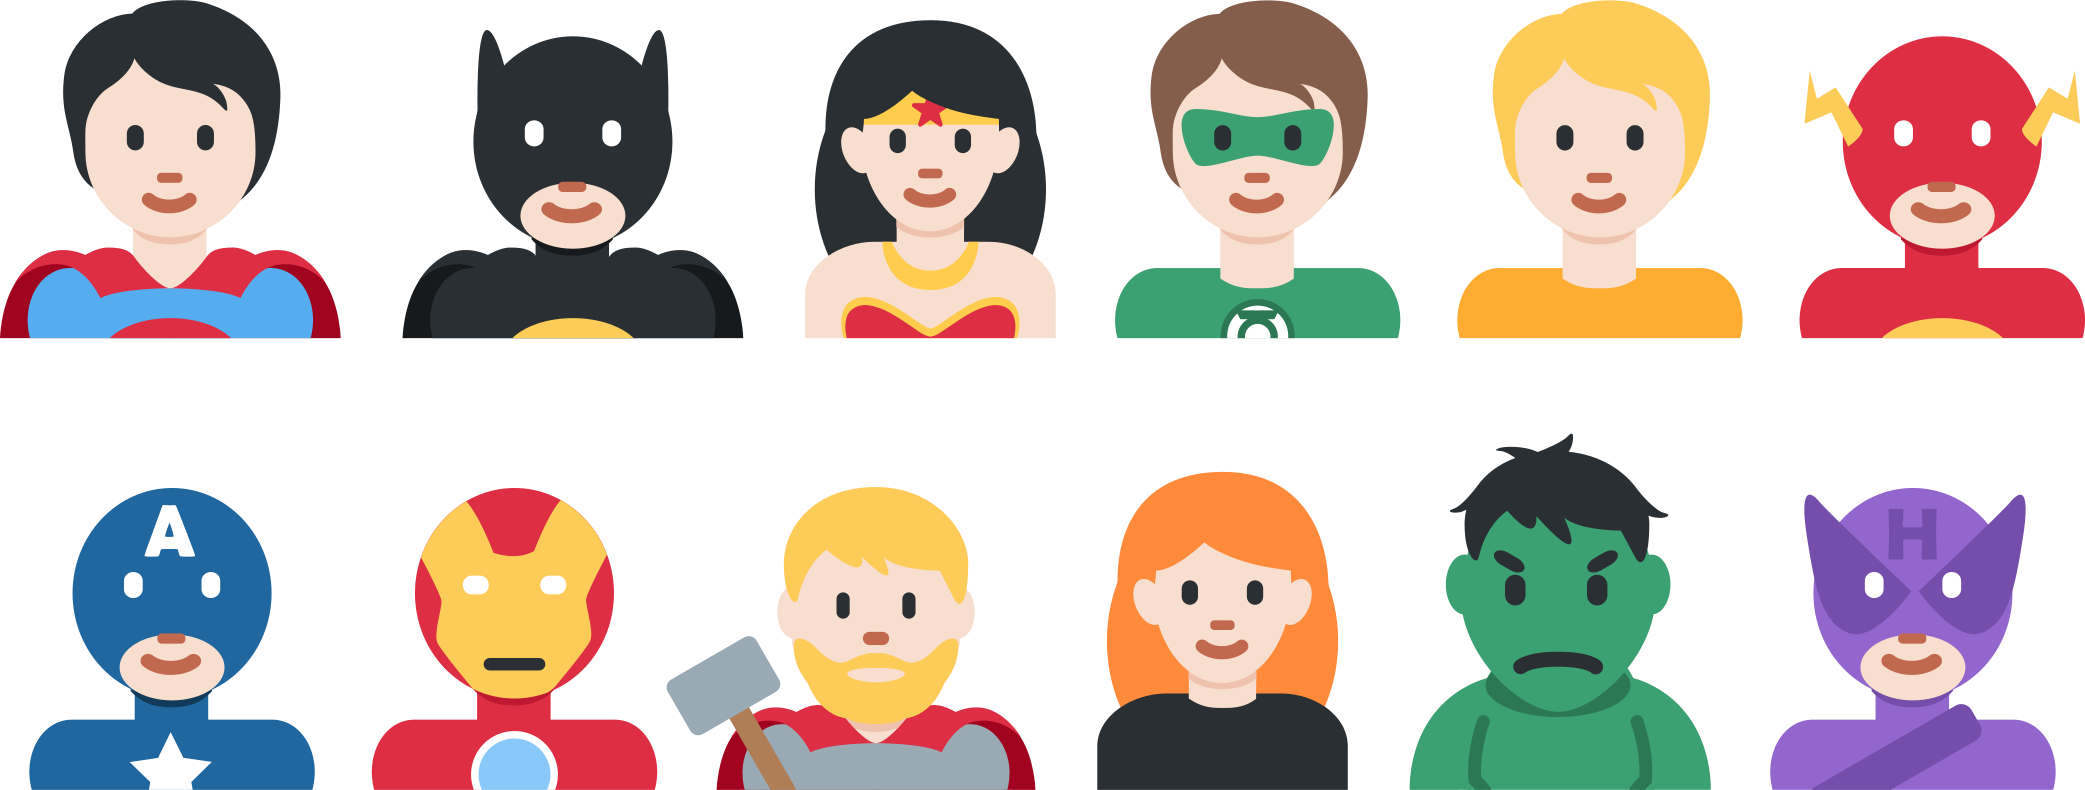
\includegraphics[width=\linewidth]{../images/Famous_superheroes.png}
		\end{columns}
	\end{frame}
	
	\section{Superman}
	
	\begin{frame}{Who is Superman?}
		\begin{columns}
			\column{0.6\textwidth}
			
\includegraphics[width=\linewidth]{../images/superhero.png}
			
			\column{0.4\textwidth}
			\lipsum[1][1-2] \\
			\vspace{1em}
			\lipsum[3][3]
			
		\end{columns}
	\end{frame}
	
	
	\begin{frame}{Who is Superman? Cont...}
		\lipsum[4][7-10] \\
		\vspace{1em}
		\lipsum[1][4-8]
	\end{frame}
	
	
	\begin{frame}
		\printbibliography
	\end{frame}
	
	\section{Thank You.}
	
	
\end{document}